\section{Versuchsdurchführung}

\subsection{Kalibrierung des Aufbaus}
\label{sub:calibration}

Vor Durchführung der Messungen wird die Winkeleinstellung des Polarisators kalibriert
und der Strom der Helmholtz-Spulen so eingestellt,
dass Störmagnetfelder in z-Richtung kompensiert werden.

Das Kalibrierungskriterium für die Winkeleinstellungen ('0$^\circ$'-Position und '90$^\circ$'-Position)
ist die Symmetrie des Hanle-Signals und die Differenz zwischen
der Höhe des rechts- und des linksseitigen Untergrundes.
Die Lage der beiden Einstellungen wird grob abgeschätzt (um -20$^\circ$ und um 70$^\circ$)
und dann in 2$^\circ$-Schritten die Hanle-Signale aufgezeichnet.
\autoref{img:durchf:winkel} zeigt zwei der gemessenen
Signale. Auf der ersten Abbildung ist die Asymmetrie deutlich zu erkennen,
auf der zweiten Abbildung ist das Signal fast symmetrisch.
Folgende Winkel wurden für '0$^\circ$'-, '45$^\circ$'- und '90$^\circ$'-Position gewählt:
\begin{equation}
\label{eq:calang}
 \varphi_0=\text{-}18^\circ, \qquad \varphi_{45}=21^\circ, \qquad \varphi_{90}=66^\circ
\end{equation}
\begin{figure}[H]
\begin{center}
  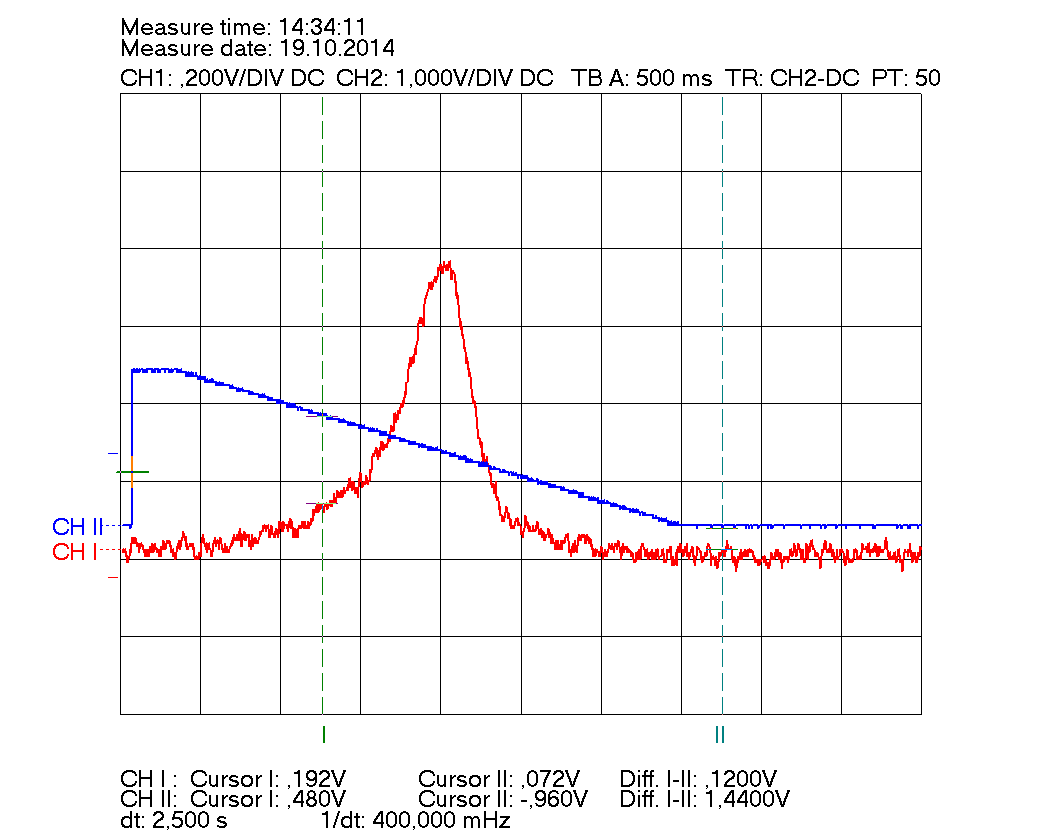
\includegraphics[width=0.49\textwidth]{../data/1/-7_5.png}
  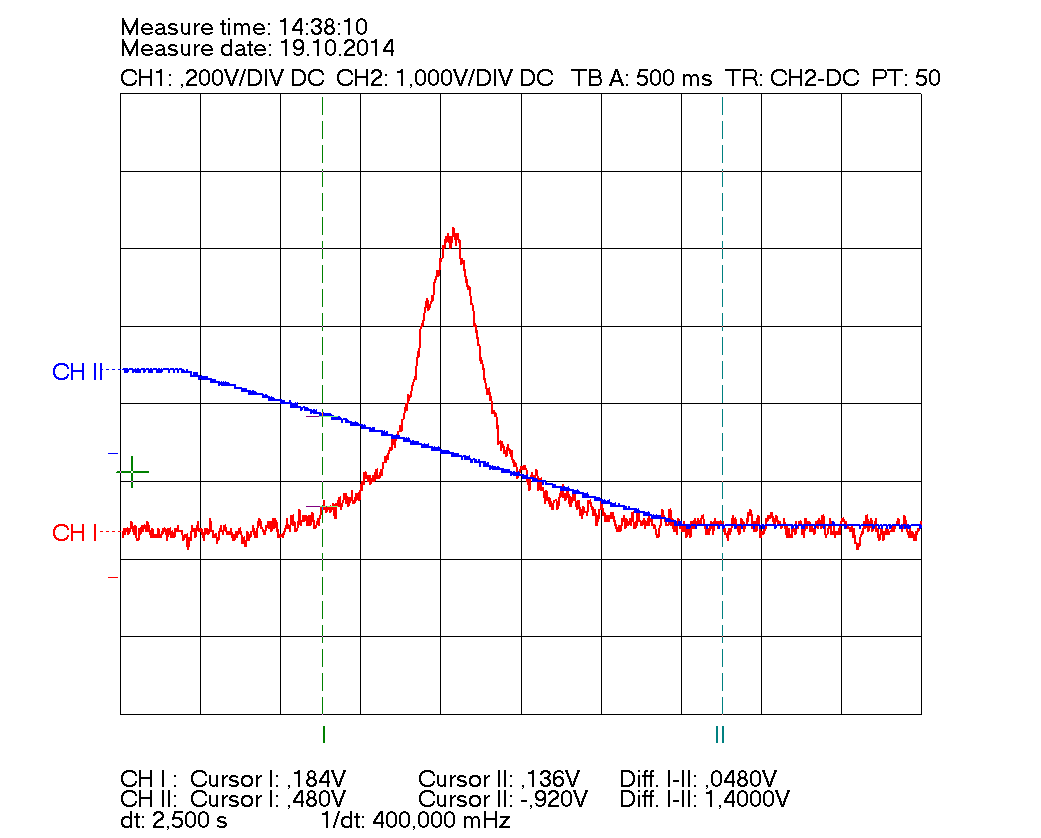
\includegraphics[width=0.49\textwidth]{../data/1/-20.png}
  \caption{Asymmetrisches Hanle-Signal bei $\varphi=\text{-}8^\circ$ (links) und
  annähernd symmetrisches Signal bei $\varphi=\text{-}20^\circ$ (rechts).}
  \label{img:durchf:winkel}
\end{center}
\end{figure}
Der Kompensationsstrom der Spulen wird eingestellt, indem die Breite des Hanle-Signals und
(in der 90$^\circ$-Position) die Signalintensität minimiert werden.
Es wird ebenfalls zuerst die korrekte Einstellung grob abgeschätzt (um -250\,mA)
und dann das Signal für mehrere Einstellungen aufgezeichnet.
Zwei Signale sind auf \autoref{img:durchf:strom} gezeigt:
Für $I_z$=400\,mA ist das Signal deutlich breiter als für $I_z$=175\,mA.
Als Kompensationsstrom wurden 
\begin{equation}
\label{eq:calcurr}
 I_z=280\,\text{mA} \qquad \text{und} \qquad I_y=0\,\text{mA}
\end{equation}
gewählt. (In y-Richtung wurde keine Kompensation durchgeführt,
da hier keine Abhängigkeit der Messergebnisse besteht.)
\begin{figure}[H]
\begin{center}
  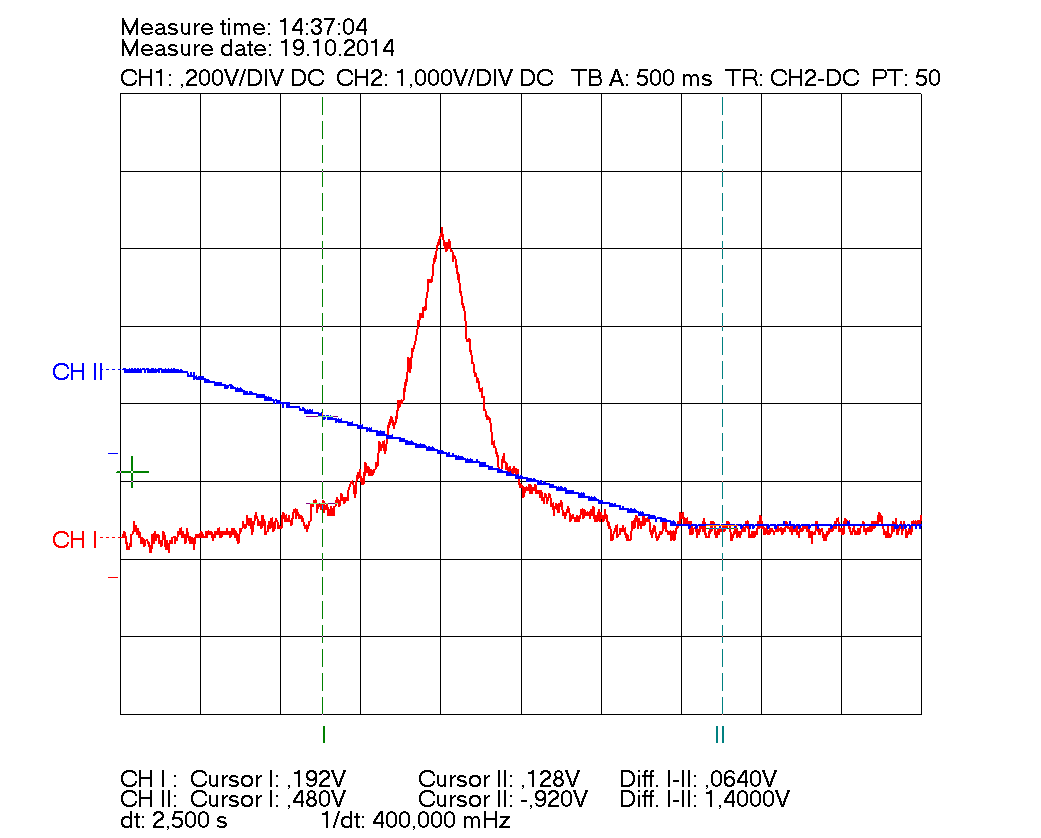
\includegraphics[width=0.49\textwidth]{../data/2/-17_5X-40.png}
    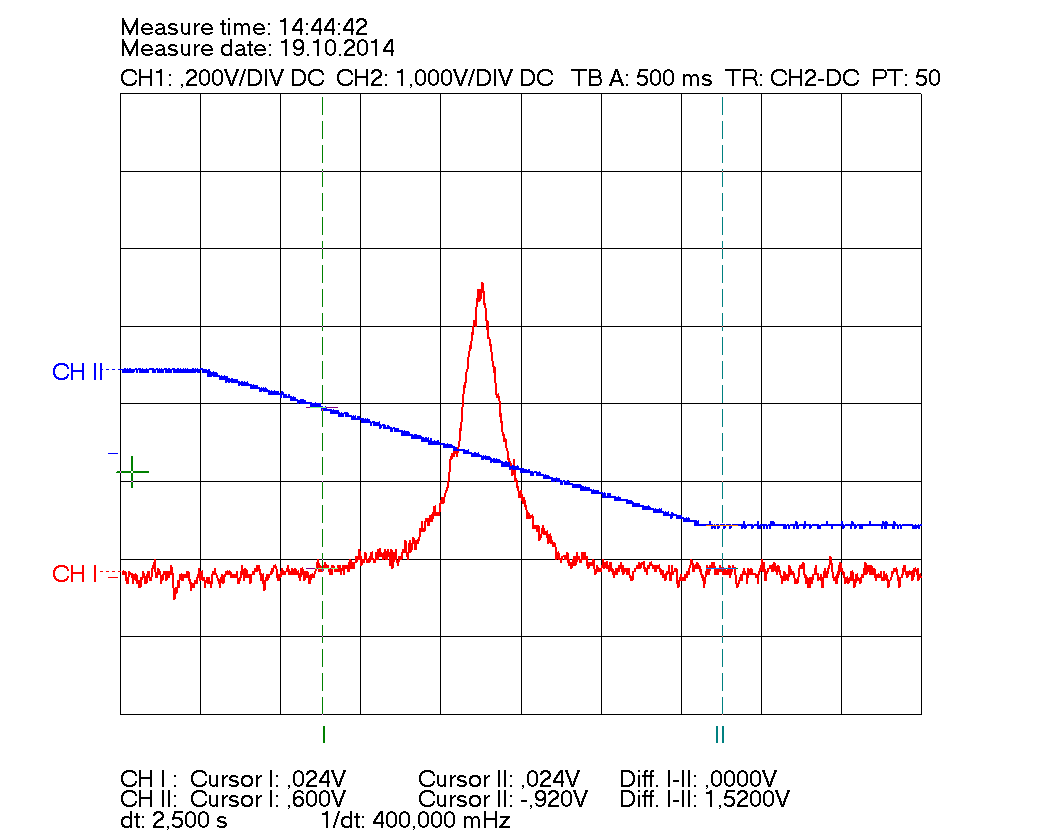
\includegraphics[width=0.49\textwidth]{../data/2/-17_5X-27_5.png}
  \caption{Breites Hanle-Signal bei $I_z=$ -400\,mA (links) und schmales Signal bei $I_z$= -275\,mA (rechts).}
  \label{img:durchf:strom}
\end{center}
\end{figure}



\subsection{Messung des Hanle-Signals}

Für die Messung des Hanle-Signals wird die Temperatur am Aufbau schrittweise abgesenkt.
Am Netzteil des Peltierelements wird dazu eine Spannung eingestellt, nach 30 Minuten Abkühlzeit
die gemessene Temperatur notiert und Messungen mit den drei oben gewählten Winkeleinstellungen durchgeführt.


